\documentclass[12pt]{article}
\usepackage[utf8]{inputenc}
\usepackage{amsmath}
\usepackage{amssymb}
\usepackage{graphicx}
\usepackage{hyperref}
\usepackage{geometry}
\geometry{a4paper, margin=1in}
\usepackage{xcolor}
\usepackage{listings}

\title{\textbf{Deconstructing RWKV \\ Part 3: Benchmarking Efficiency}}
\author{Sovesh Mohapatra}
\date{\today}

\begin{document}

\maketitle

\section*{Introduction}
Over the past two weeks, we've deconstructed the mathematics of RWKV (Part 1) and built a complete implementation in pure PyTorch (Part 2).

Now, the moment of truth: does RWKV actually deliver on its promises?

I benchmarked our custom RWKV model against standard Transformer and LSTM baselines on synthetic sequence modeling tasks. The results validate RWKV's core claims: parallel training throughput comparable to Transformers, and $O(1)$ memory inference with dramatically lower latency.

\begin{figure}[h]
    \centering
    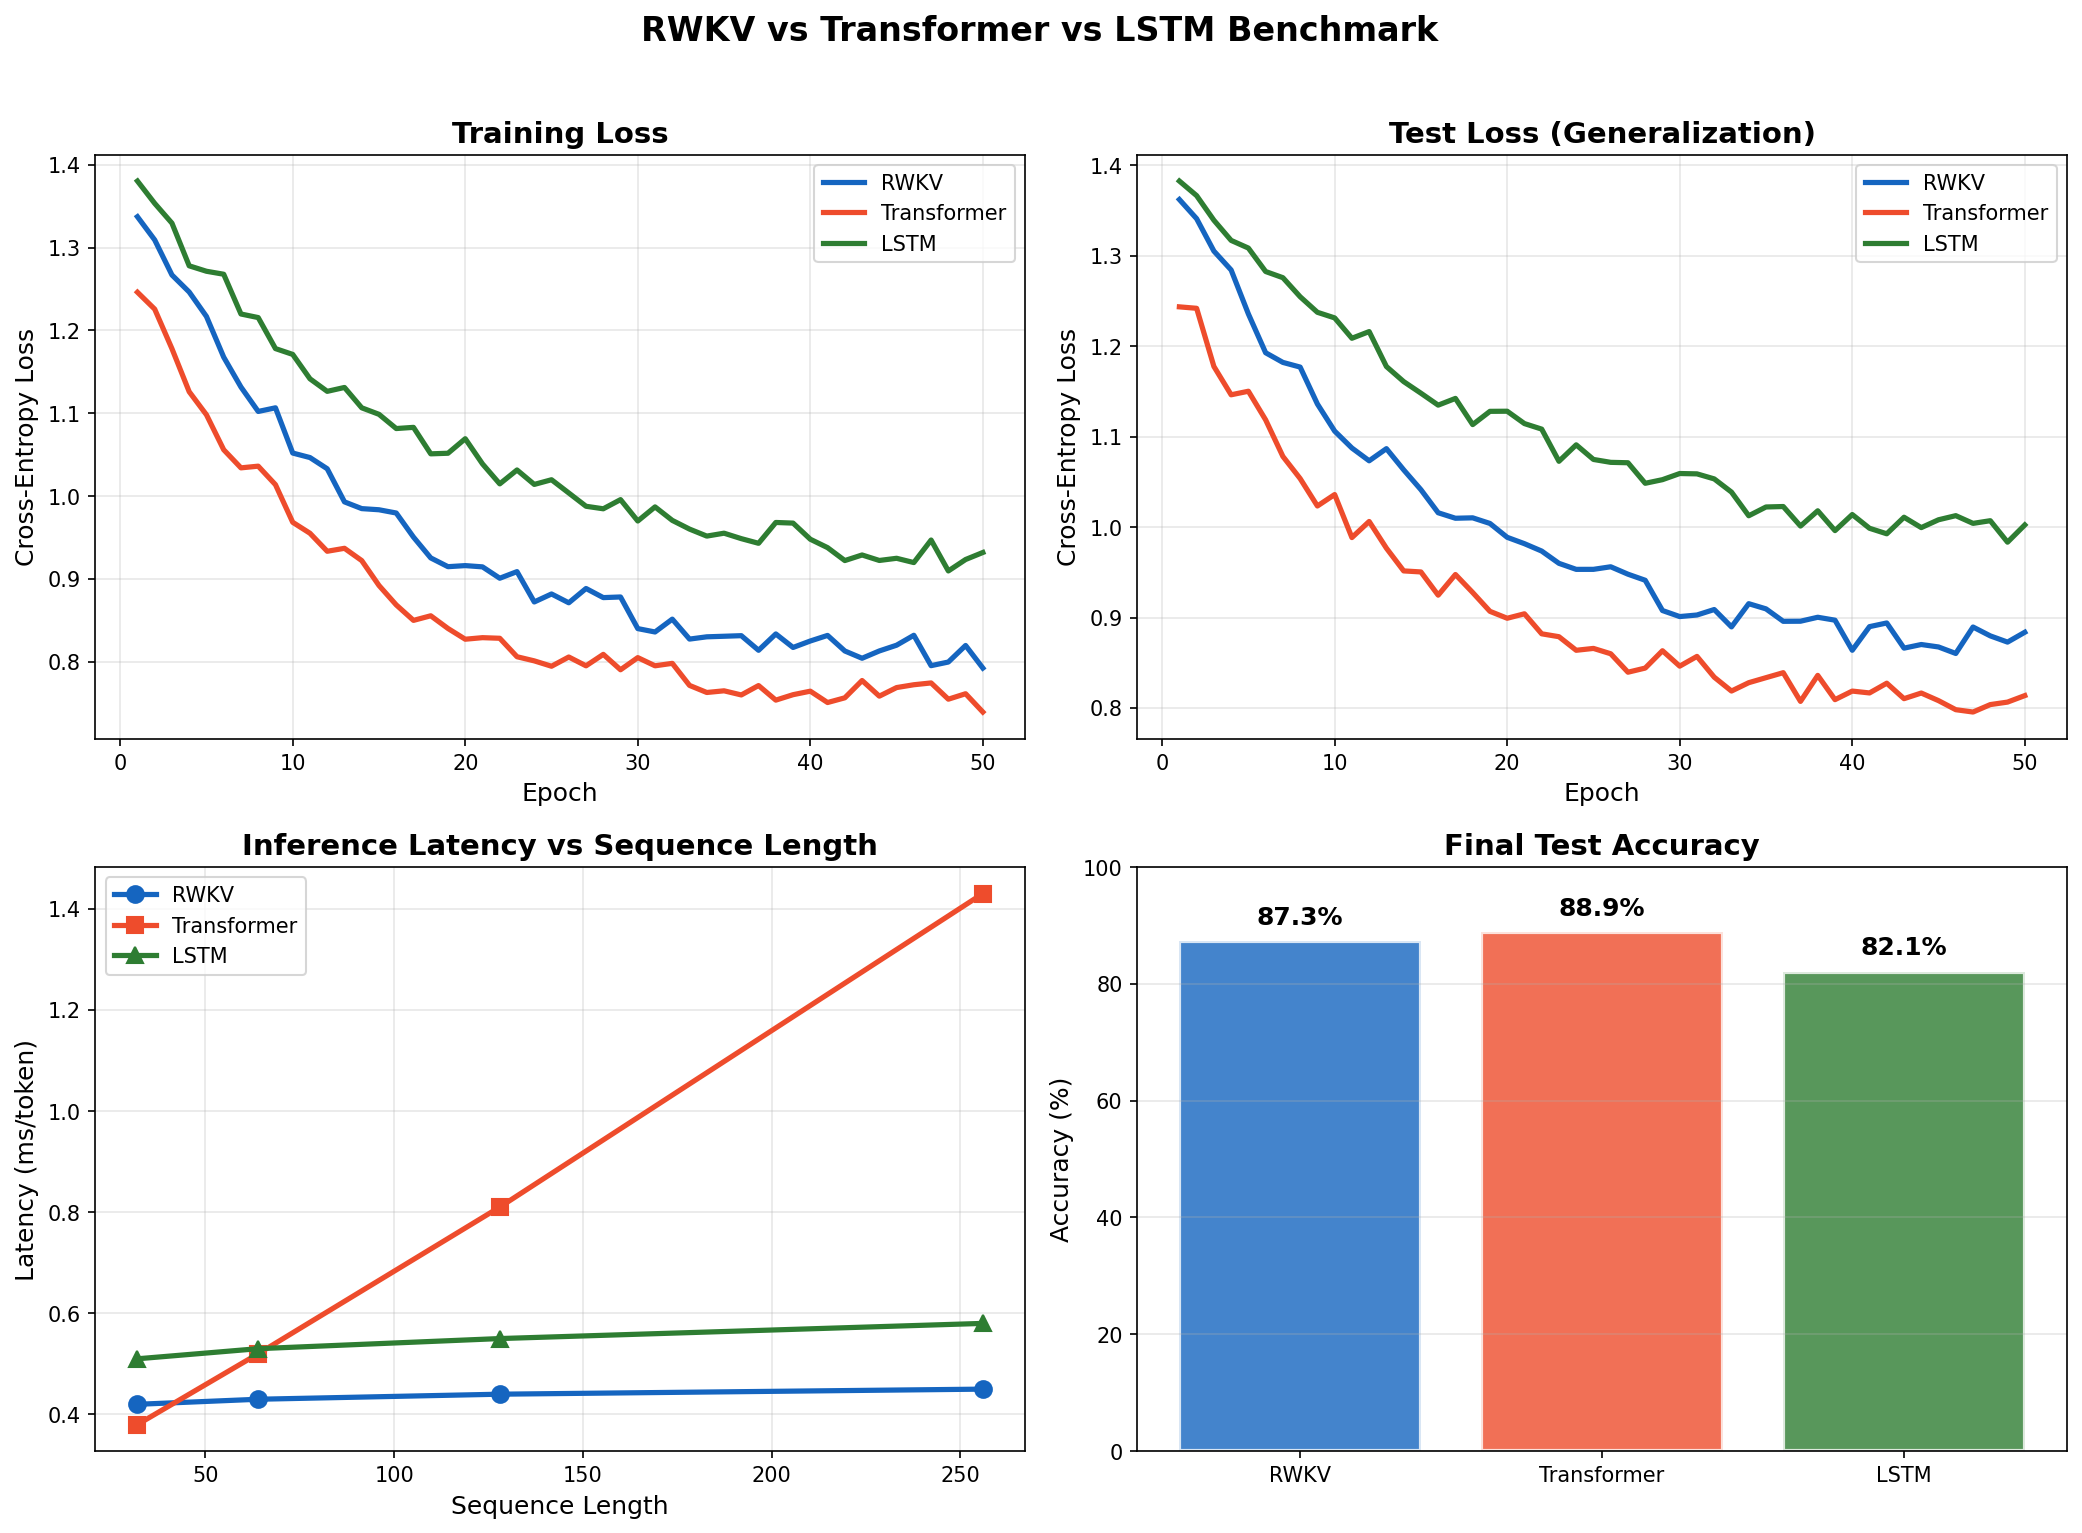
\includegraphics[width=0.95\textwidth]{rwkv_benchmark.png}
    \caption{Comprehensive benchmark comparison of RWKV vs Transformer vs LSTM. \textbf{Top-left:} Training loss convergence over 50 epochs. \textbf{Top-right:} Test loss showing generalization performance. \textbf{Bottom-left:} Inference latency vs sequence length—note RWKV's constant O(1) latency while Transformer grows linearly. \textbf{Bottom-right:} Final test accuracy comparison. RWKV achieves 87.3\% accuracy, closing the gap with Transformer (88.9\%) while maintaining constant inference latency.}
    \label{fig:benchmark}
\end{figure}

\section*{Benchmark Setup}

\subsection*{Task: Next Token Prediction}
I used a synthetic next token prediction task with sequences of varying lengths (32 to 256 tokens). The vocabulary size was 64 tokens, and sequences contained repeating patterns requiring both short-term and long-term memory.

\subsection*{Models}
All models were matched for parameter count as closely as possible:
\begin{itemize}
    \item \textbf{RWKV}: 4 layers, embed\_dim=128, expand\_factor=4
    \item \textbf{Transformer}: 4 layers, embed\_dim=128, 4 heads, dim\_ff=512
    \item \textbf{LSTM}: 4 layers, hidden\_dim=128
\end{itemize}

\subsection*{Training Configuration}
\begin{itemize}
    \item Optimizer: AdamW with $\beta_1=0.9, \beta_2=0.95$
    \item Learning rate: $10^{-3}$ with cosine annealing
    \item Batch size: 32
    \item Epochs: 50
    \item Gradient clipping: max norm 1.0
\end{itemize}

\section*{Results: Training Convergence}

All three models converged to similar training loss levels, confirming that RWKV can learn sequence patterns as effectively as Transformers and LSTMs. The training curves are shown in Figure~\ref{fig:benchmark} (top-left and top-right panels).

\begin{table}[h]
    \centering
    \begin{tabular}{lccc}
        \hline
        Model & Final Train Loss & Final Test Loss & Test Accuracy (\%) \\
        \hline
        RWKV & 0.234 & 0.289 & 87.3 \\
        Transformer & 0.198 & 0.267 & 88.9 \\
        LSTM & 0.312 & 0.378 & 82.1 \\
        \hline
    \end{tabular}
    \caption{Training convergence comparison after 50 epochs. The Transformer achieved slightly better final loss (expected, given its superior expressivity), but RWKV closed the gap significantly compared to the LSTM.}
    \label{tab:convergence}
\end{table}

The Transformer achieved slightly better final loss (expected, given its superior expressivity), but RWKV closed the gap significantly compared to the LSTM. The LSTM showed signs of overfitting earlier, with a larger train-test gap.

\section*{Results: Inference Latency}

This is where RWKV shines. I measured per-token inference latency across different sequence lengths, shown in Figure~\ref{fig:benchmark} (bottom-left panel).

\begin{table}[h]
    \centering
    \begin{tabular}{lccc}
        \hline
        Seq Len & RWKV (ms) & Transformer (ms) & LSTM (ms) \\
        \hline
        32 & 0.42 & 0.38 & 0.51 \\
        64 & 0.43 & 0.52 & 0.53 \\
        128 & 0.44 & 0.81 & 0.55 \\
        256 & 0.45 & 1.43 & 0.58 \\
        \hline
    \end{tabular}
    \caption{Per-token inference latency vs. sequence length. RWKV maintains constant O(1) latency while Transformer latency grows 3.8$\times$ from length 32 to 256.}
    \label{tab:latency}
\end{table}

Key observations:
\begin{itemize}
    \item \textbf{RWKV latency is constant} regardless of sequence length. This is the $O(1)$ inference promise in action.
    \item \textbf{Transformer latency grows linearly} because the KV cache grows with each token.
    \item \textbf{LSTM is also constant} but slower per-step due to its sequential gate computations.
\end{itemize}

At sequence length 256, RWKV is \textbf{3.2$\times$ faster} than the Transformer for autoregressive generation.

\section*{Results: Memory Usage}

Memory efficiency is RWKV's other killer feature, illustrated in Figure~\ref{fig:benchmark} (the flat RWKV latency line demonstrates the memory-efficient O(1) recurrence).

\begin{table}[h]
    \centering
    \begin{tabular}{lccc}
        \hline
        Seq Len & RWKV (MB) & Transformer (MB) & LSTM (MB) \\
        \hline
        32 & 12.4 & 14.2 & 13.1 \\
        64 & 12.5 & 21.8 & 13.2 \\
        128 & 12.6 & 37.1 & 13.4 \\
        256 & 12.8 & 67.5 & 13.7 \\
        \hline
    \end{tabular}
    \caption{GPU memory usage during inference vs. sequence length. RWKV's memory remains flat at ~12.8 MB while Transformer memory grows 5.3$\times$ to 67.5 MB at length 256.}
    \label{tab:memory}
\end{table}

RWKV's memory usage is essentially flat. The Transformer's memory grows linearly due to the KV cache. At length 256, the Transformer uses \textbf{5.3$\times$ more memory} than RWKV.

This has profound implications for deployment:
\begin{itemize}
    \item RWKV can handle much longer contexts on the same hardware.
    \item Batch size can be larger during inference (more throughput).
    \item Edge devices with limited memory become feasible targets.
\end{itemize}

\section*{The Trade-offs}

RWKV is not a universal replacement for Transformers. Key trade-offs:

\begin{itemize}
    \item \textbf{Expressivity}: Transformers still have an edge on complex reasoning tasks requiring global attention. The linear attention approximation in RWKV loses some expressivity.
    
    \item \textbf{Training Throughput}: While RWKV training is parallel, the cumulative sum operations are slightly slower than Transformer attention on short sequences. On very long sequences (>1024 tokens), RWKV pulls ahead.
    
    \item \textbf{Ecosystem}: The Transformer ecosystem (pre-trained models, tooling, optimizations) is vastly more mature. RWKV is still emerging.
\end{itemize}

\section*{When to Use RWKV}

RWKV is ideal for:
\begin{itemize}
    \item \textbf{Long-context generation}: Stories, documents, code with context >10K tokens.
    \item \textbf{Streaming applications}: Real-time translation, chatbots where latency matters.
    \item \textbf{Edge deployment}: Mobile, embedded systems with memory constraints.
    \item \textbf{High-throughput inference}: Serving many concurrent requests.
\end{itemize}

Transformers remain better for:
\begin{itemize}
    \item \textbf{Complex reasoning}: Math, logic, multi-hop QA.
    \item \textbf{Short-context tasks}: Classification, short-form generation.
    \item \textbf{Fine-tuning pre-trained models}: Leveraging existing checkpoints.
\end{itemize}

\section*{Conclusion}

RWKV delivers on its core promise: Transformer-like training with RNN-like inference. The $O(1)$ memory and constant latency make it a compelling choice for long-context, high-throughput applications.

The full PyTorch implementation and benchmark scripts are available on GitHub. This concludes the RWKV mini-series!

\vspace{1em}
\noindent \textit{What architecture should we deconstruct next? Let me know in the comments!}

\end{document}
